\tikzset{
  every picture/.style={line width=0.75pt}, % Set default line width
  every node/.style={text=foreground}, % Set default node text color
  every path/.style={color=linecolor}, % Set default line color
}

\tikzsetnextfilename{overview}%
\begin{tikzpicture}

  \begin{scope}[spy using outlines={magnification=2,size=12mm,very thick, draw=funkey_color_1}]

    \node[image] (frame) {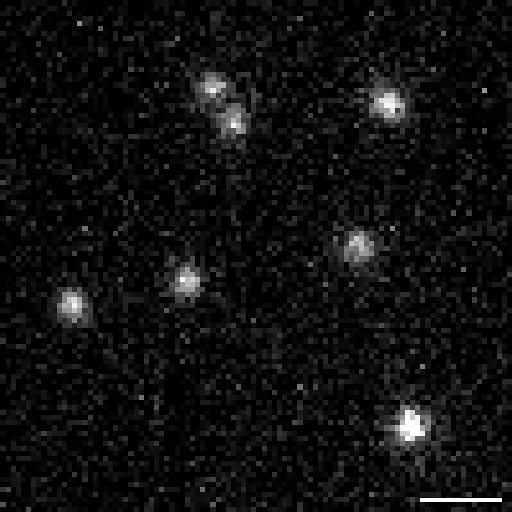
\includegraphics[width=42mm]{figures/data/overview/sample_frame}};

    \spy on ($(frame)+(1.1, 1.2)$)
      in node (patch_3) [image,right=6mm,anchor=north west]
      at (frame.north east);
    \spy on ($(frame)+(0.9, 1.1)$)
      in node (patch_2) [image,right=6mm,anchor=north west]
      at ($(frame.north east)-(0.1,0.1)$);
    \spy[
        draw=funkey_color_1,
        every spy on node/.append style={ultra thick},
        every spy in node/.append style={ultra thick},
        spy connection path={\draw[ultra thick, color=funkey_color_1] (tikzspyonnode) -- (tikzspyinnode);}
    ]
      on ($(frame)+(1.1, 1.25)$)
      in node (patch_1) [image,right=6mm,anchor=north west]
      at ($(frame.north east)-(0.2,0.2)$);
  \end{scope}

  % Example trace
  \begin{scope}
    \def\tracecsv{figures/data/overview/trace.csv}
    \def\traceintensitycol{trace}
    \def\nolabels{}
    \setlength\plotwidth{64mm}
    \setlength\plotheight{20mm}
    \pgfplotsset{every axis/.style={
      xshift=6mm,
      anchor=north west,
      name=trace,
      at={(patch_3.north east)},
      tick label style={color=foreground},
      axis line style={color=foreground}
    }}
    \@ifundefined{nolabels}{
  \pgfplotsset{xlabel=frames}
  \pgfplotsset{ylabel=intensity}
  \pgfplotsset{grid=major}
  \pgfplotsset{grid style={dashed}}
}{
  \pgfplotsset{xticklabel=\empty}
  \pgfplotsset{yticklabel=\empty}
  \pgfplotsset{ticks=none}
  \pgfplotsset{scaled ticks=false}
}
\@ifundefined{histogramcsv}{}{
  \setlength{\plotwidth}{0.73\plotwidth}
}
\begin{axis}[
  name=trace,
  width=\plotwidth,
  height=\plotheight,
  scale only axis=true,
  enlarge x limits=false,
  xtick distance=500,
  ticklabel style={font=\small},
  legend style={fill=black, nodes={scale=0.6, transform shape}},
]

  \addplot [
    color=tracecolor,
    mark=*,
    mark size=0.7pt,
    mark options={line width=0},
    fill opacity=0.8,
    draw opacity=0.0,
  ] table [
    col sep=comma,
    x=frames,
    y=\traceintensitycol
  ] {\tracecsv};
  \@ifundefined{nolabels}{\addlegendentry{intensity trace}}{}

  \@ifundefined{zcol}{}{
    \addplot [
      color=ztracecolor,
      thick
    ] table [
      col sep=comma,
      x=frames,
      y=\zcol
    ] {\tracecsv};
    \@ifundefined{nolabels}{\addlegendentry{inferred state}}{}
  }

  % remember min/max y-axis values for next plot
  \pgfplotsextra{
    \pgfmathparse{\pgfkeysvalueof{/pgfplots/ymin}}
    \global\let\ymin\pgfmathresult
    \pgfmathparse{\pgfkeysvalueof{/pgfplots/ymax}}
    \global\let\ymax\pgfmathresult
  }

\end{axis}
\@ifundefined{plotlabel}{}{
  \node[anchor=north west,rectangle,draw,fill=black] at (trace.north west) {\plotlabel};
}

\@ifundefined{histogramcsv}{}{
  \begin{axis}[
    at={($(trace.east) + (4mm,0)$)},
    name=histogram,
    anchor=west,
    width=0.25\plotwidth,
    height=\plotheight,
    scale only axis=true,
    ylabel=\empty,
    yticklabel=\empty,
    xtick distance=0.01,
    xlabel=probability,
    grid=major,
    grid style={dashed, very thin},
    enlarge x limits={value=0.4,upper},
    scaled ticks=false,
    ymin=\ymin,
    ymax=\ymax,
    ticklabel style={font=\small},
    legend style={fill=black, nodes={scale=0.6, transform shape}},
  ]

    \addplot+[
      xbar interval,
      mark=none,
      color=tracecolor,
      fill=tracecolor,
      fill opacity=0.6,
      draw=none,
    ] table [
      col sep=comma,
      y=\histbincol,
      x=\histcountcol,
    ] {\histogramcsv};
    \addlegendentry{intensity histogram}

    \addplot[
      color=intensitymodelcolor!80!black,
      thick
    ] table [
      col sep=comma,
      y=\histbincol,
      x=\modelfitcol
    ] {\histogramcsv};
    \addlegendentry{inferred model}

  \end{axis}
}

  \end{scope}

  \node[anchor=north,inner sep=2pt,color=foreground] at (trace.230) {\small time};
  \node[rotate=90,anchor=south,inner sep=2pt,color=foreground] at (trace.west) {\small intensity};

  % Observed / hidden line
  \draw[color=linecolor,very thick]
    (patch_1.west|-frame.350) --
      node[pos=0,anchor=south west,color=foreground] {observed}
      node[pos=0,anchor=north west,color=foreground] {hidden}
      node[pos=0.36] (sample_1) {}
      node[pos=0.62] (sample_2) {}
      node[pos=0.95] (sample_3) {}
    (trace.east|-frame.350);

  % Brace to MLE
  \draw[color=linecolor,decorate,decoration={brace,raise=2mm,aspect=0.2}]
    (trace.north east) --
    node[pos=0.2,right=2mm] (brace) {}
       node[pos=0.1,right=14mm,draw,rectangle,rounded corners] (sparkles) {\textit{sparkles}}
       node[pos=0.5,right=16mm,draw,rectangle,rounded corners] (mle) {\ours}
    (trace.south east);

  % Posterior
  \begin{scope}
    \def\posteriorcsv{figures/data/overview/posterior.csv}
    \def\posteriorcol{posterior}
    \def\noylabels{}
    \setlength\plotwidth{24mm}
    \setlength\plotheight{24mm}
    \pgfplotsset{every axis/.style={
      yshift=-8mm,
      anchor=north,
      name=posterior,
      at=(mle),
      tick label style={color=foreground},
      axis line style={color=foreground}
    }}
    \def\eps{0.001}%  skip bars for values below eps
\@ifundefined{noylabels}{}{
  \pgfplotsset{yticklabel=\empty}
  \pgfplotsset{ylabel=\empty}
}
\@ifundefined{noxlabel}{
  \pgfplotsset{xlabel=$n$}
}{
  \pgfplotsset{xlabel=\empty}
}
\begin{axis}[
  width=\plotwidth,
  height=\plotheight,
  scale only axis=true,
  enlarge x limits={abs=1.5},
  enlarge y limits=0,
  ymin=0,
  ymax=1,
  scaled ticks=false,
  ticklabel style={font=\tiny},
  xtick distance=1,
  axis background/.style={fill=white},
]

  \addplot+[
    ybar,
    bar width=1,
    mark=none,
    fill=posteriorcolor,
    fill opacity=0.6,
    draw=posteriorcolor,
    y filter/.expression={
      y < \eps ? nan : y
    },
  ] table [
    col sep=comma,
    y=\posteriorcol,
    x=n,
  ] {\posteriorcsv};

  \ifdefined\posteriorcolextra
    \addplot+[
      ybar,
      bar width=1,
      mark=none,
      fill=posteriorcolor!60!black,
      fill opacity=0.6,
      draw=posteriorcolor,
      y filter/.expression={
        y < \eps ? nan : y
      },
    ] table [
      col sep=comma,
      y=\posteriorcolextra,
      x=n,
    ] {\posteriorcsv};
  \fi

\end{axis}

  \end{scope}

  \draw[color=linecolor,arrow] (brace) -- (sparkles);
  \draw[color=linecolor,arrow] (sparkles) -- (mle);

  \draw[color=linecolor,arrow] (brace) -- (mle);
  \draw[color=linecolor,arrow] (mle) -- (posterior);

  % Blinky things
  \node (hidden) at (frame.326-|patch_1) {\blinky{off}{off}{off}{off}{off}};
  \node (z_sample_1) at (frame.326-|sample_1) {\blinky{on}{off}{on}{on}{off}};
  \node (z_sample_2) at (frame.326-|sample_2) {\blinky{on}{off}{on}{off}{off}};
  \node (z_sample_3) at (frame.326-|sample_3) {\blinky{on}{off}{off}{off}{off}};

  \draw[color=linecolor,arrow] (z_sample_1) -- +(0, 2.8);
  \draw[color=linecolor,arrow] (z_sample_2) -- +(0, 2.4);
  \draw[color=linecolor,arrow] (z_sample_3) -- +(0, 2.0);

  \node[anchor=north,inner sep=10pt,color=foreground] at (hidden) {\strut$\n=5$};
  \node[anchor=north,inner sep=10pt,color=foreground] at (z_sample_1) {\strut$\z{}=3$};
  \node[anchor=north,inner sep=10pt,color=foreground] at (z_sample_2) {\strut$\z{}=2$};
  \node[anchor=north,inner sep=10pt,color=foreground] at (z_sample_3) {\strut$\z{}=1$};

\end{tikzpicture}

